\chapter{Thử nghiệm và kết quả}
\section{Mục đích và cách tiến hành}
Nhóm em chia quá trình thử nghiệm thành ba phần. Đầu tiên, nhóm xây dựng baseline pixel và so sánh với HOG ở V1. Sau đó, nhóm bổ sung đặc trưng màu và PCA trong V2. Cuối cùng, nhóm kiểm tra độ ổn định trên các fold lấy từ train và quan sát đường học. Các số trong phần này được lấy từ những lần chạy thực tế đã được lưu và kiểm tra trước khi nhóm yêu cầu xóa output; các thành viên cần chạy lại để tạo tệp kết quả mới. Nhóm không tạo thêm điểm test E6.

Với V1 và V2, mỗi cấu hình được fit trên train và đánh giá trên validation chính thức. V2 có 56 cấu hình được xét. Cấu hình tốt nhất trong mỗi nhóm được chọn theo F1 trung bình vĩ mô trên validation, sau đó là Accuracy. Vì validation được dùng nhiều lần để lựa chọn, điểm của cấu hình thắng có thể lạc quan và chưa phải kết quả đánh giá trên dữ liệu hoàn toàn mới.
\section{So sánh sáu thí nghiệm trên validation}
Bảng \ref{tab:val} chép số liệu từ \texttt{results/v2/metrics/comparison.json}. Mục đích của E1 là tạo một mức cơ sở dễ giải thích; E2 và E3 dùng HOG để xem đặc trưng cạnh kết hợp K-NN hoặc cây quyết định như thế nào. E4 bổ sung màu; E5 giảm chiều pixel; E6 kết hợp màu với PCA.
\begin{table}[htbp]\centering\begin{tabular}{llrr}\toprule
ID & Đặc trưng và mô hình & Accuracy & Macro F1\\\midrule
E1 & Pixel + K-NN & 0,1088 & 0,0914\\
E2 & HOG + K-NN & 0,0608 & 0,0584\\
E3 & HOG + cây quyết định & 0,0245 & 0,0230\\
E4 & HOG + HSV + K-NN & 0,2186 & 0,2003\\
E5 & Pixel + PCA + K-NN & 0,1500 & 0,1334\\
E6 & HOG + HSV + PCA + K-NN & 0,2343 & 0,2127\\\bottomrule
\end{tabular}\caption{Kết quả tốt nhất mỗi nhóm trên validation chính thức.}\label{tab:val}\end{table}
\hinh{validation.png}{0.78}{So sánh F1 vĩ mô của E1–E6 trên validation chính thức.}

Trong sáu kết quả này, E6 có F1 validation cao nhất: 0,2127. Mức tăng so với E1 là khoảng 0,1212 điểm tuyệt đối; so với E4 là khoảng 0,0124. Kết quả thấp nhất là E3, đạt 0,0230. Kết quả này cho thấy cấu hình cây quyết định đã thử không phù hợp bằng các cấu hình còn lại trên validation, nhưng không có nghĩa mọi cây quyết định đều kém trong mọi bài toán.
\section{Kiểm định chéo trên train}
Để không chỉ dựa vào một lần chia train/validation, nhóm em dùng năm fold phân tầng được tạo từ 1.020 ảnh train chính thức. Với mỗi fold, 816 ảnh dùng để fit và 204 ảnh còn lại dùng để kiểm tra; mỗi lớp có hai ảnh trong phần kiểm tra fold. Các cấu hình E1, E4 và E6 đều dùng cùng fold để việc so sánh công bằng hơn. Validation chính thức và test không tham gia quá trình này.

Trung bình ± độ lệch chuẩn quần thể của F1 vĩ mô giữa năm fold lần lượt là E1 0,0877 ± 0,0118; E4 0,1852 ± 0,0148; E6 seed PCA 42 là 0,1932 ± 0,0195. Khi giữ nguyên fold và thay seed PCA của E6, trung bình thu được là 0,1958 với seed 7 và 0,1970 với seed 123. Độ lệch giữa fold chỉ mô tả biến thiên trong phép thử này, không phải khoảng tin cậy. Ngoài ra, ba cấu hình đã được lựa chọn dựa trên validation trước khi chạy CV, nên kết quả CV không đánh giá toàn bộ quá trình tìm cấu hình.
\hinh{kiem_dinh_cheo.png}{0.78}{F1 vĩ mô trên năm fold của train; thanh sai số là độ lệch chuẩn giữa fold.}
\section{Đường học và kiểm tra khoảng cách giữa train và fold giữ lại}
Do K-NN không huấn luyện theo epoch như mạng nơ-ron, nhóm em không vẽ đường theo số epoch. Thay vào đó, nhóm dùng các tập con có 2, 4, 6 và 8 ảnh mỗi lớp trong phần train của từng fold, tương ứng 204, 408, 612 và 816 ảnh. Tập con được chọn phân tầng và lồng nhau; E1, E4 và E6 dùng cùng mẫu ở mỗi mức. Phần giữ lại của mỗi fold luôn gồm 204 ảnh, không xuất hiện trong phép fit. PCA của E6 được fit lại trên đúng tập con ở từng mức. Tổng cộng có 60 lần fit thực tế: ba mô hình × bốn mức dữ liệu × năm fold.

\begin{table}[htbp]\centering\begin{tabular}{rrrr}\toprule
Ảnh fit & E1 & E4 & E6\\\midrule
204 & 0,0476 & 0,1259 & 0,1306\\
408 & 0,0688 & 0,1548 & 0,1520\\
612 & 0,0788 & 0,1735 & 0,1689\\
816 & 0,0877 & 0,1852 & 0,1932\\\bottomrule
\end{tabular}\caption{F1 vĩ mô trung bình trên fold giữ lại theo số ảnh fit; không phải validation chính thức hoặc test.}\label{tab:duonghoc}\end{table}
\hinh{duong_hoc.png}{0.98}{Đường học E1, E4 và E6 trên train chính thức. Vùng mờ là độ lệch chuẩn giữa năm fold của điểm holdout.}
\hinh{so_sanh_duong_hoc.png}{0.78}{So sánh F1 trung bình trên cùng fold giữ lại theo số ảnh fit.}

Ở cả ba mô hình, F1 trên tập fit đạt 1,0. Cần chú ý điểm này được tính trên chính các ảnh đã fit: với K-NN, một ảnh có thể trở thành láng giềng của chính nó, làm điểm train rất lạc quan. Vì vậy, khoảng cách lớn giữa hai đường cho thấy việc dự đoán trên ảnh đã thấy và ảnh giữ lại khác nhau nhiều, nhưng không thể dùng riêng biểu đồ để khẳng định chắc chắn nguyên nhân overfitting. Đường holdout tăng khi số ảnh fit tăng trong phép thử này. Tại mức 408 và 612 ảnh, E4 nhỉnh hơn E6; tại 816 ảnh, E6 nhỉnh hơn E4. Mỗi lớp chỉ có hai ảnh trong holdout của mỗi fold nên các chênh lệch nhỏ cần được diễn giải thận trọng.

Nhóm đã đối chiếu điểm ở mức 816 ảnh với kết quả V3 đã lưu; sai khác lớn nhất giữa các fold nhỏ hơn $10^{-12}$. Bảng từng fold, các ID mẫu được chọn và checksum đầu vào nằm trong \texttt{results/duong\_hoc/}. Không có dự đoán mới trên validation chính thức hay test trong phép thử đường học.
\section{Thời gian, bộ nhớ và ma trận nhầm lẫn}
Trong lần đo V3 trên máy cục bộ, E1 fit trung bình 0,0082 giây, dự đoán 0,0580 giây và RSS đỉnh worker 343,8 MiB; E4 lần lượt 0,0040 giây, 0,0234 giây và 214,1 MiB; E6 tính cả PCA và K-NN lần lượt 0,0278 giây, 0,0026 giây và 217,0 MiB. RSS gồm Python, thư viện, ma trận train và mảng tạm. Thời gian này không gồm trích xuất đặc trưng và có thể thay đổi theo máy.

Hình \ref{fig:cm} là ma trận nhầm lẫn E6 trên validation chính thức, không phải test. E6 có 22 lớp có F1 bằng 0; mỗi lớp validation chỉ có 10 ảnh. Hai cặp nhầm có hướng 24→11 và 94→32 xuất hiện bốn lần mỗi cặp. Việc xem ảnh lỗi giúp nhóm tìm các trường hợp cần phân tích tiếp, nhưng không tự chứng minh yếu tố nào đã gây ra lỗi.
\begin{figure}[htbp]\centering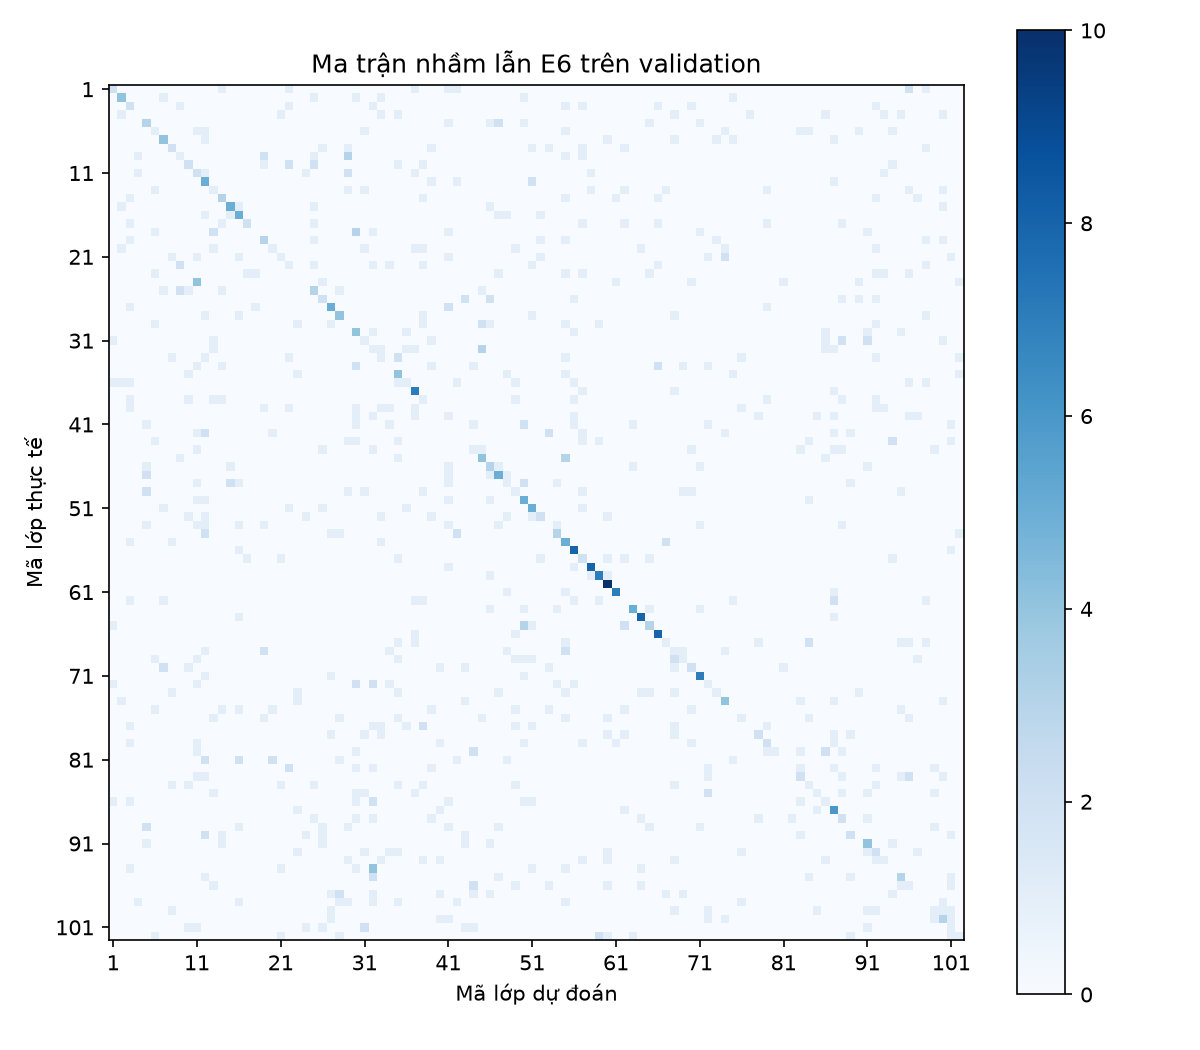
\includegraphics[width=0.67\textwidth]{figures/ma_tran_e6.png}\caption{Ma trận nhầm lẫn E6 trên validation chính thức.}\label{fig:cm}\end{figure}
\section{Diễn giải chi tiết từng nhóm thí nghiệm}
\textbf{E1 — pixel và K-NN.} Đây là baseline trực tiếp nhất: mỗi ảnh sau chuẩn hóa trở thành một vector chứa giá trị RGB. Mục đích là có một mốc so sánh trước khi thêm các phép trích xuất phức tạp hơn. E1 đạt Accuracy validation 0,1088 và F1 vĩ mô 0,0914. Điểm số cho thấy việc chỉ so sánh pixel đã nhận đúng được một phần ảnh, nhưng chưa xử lý tốt các thay đổi về bố cục, vị trí hoặc nền.

\textbf{E2 — HOG và K-NN.} Nhóm dùng HOG để xem việc mô tả cạnh và hướng gradient có giúp phân biệt hình hoa hay không. Cấu hình tốt nhất E2 đạt Accuracy 0,0608 và F1 vĩ mô 0,0584 trên validation. Với dữ liệu và lưới tham số đã thử, E2 thấp hơn E1; nhóm không loại bỏ kết quả âm này vì nó cho thấy một đặc trưng thường dùng không tự động tốt hơn pixel trong mọi bài toán.

\textbf{E3 — HOG và cây quyết định.} Cấu hình này giữ nhóm đặc trưng HOG nhưng thay bộ phân loại, giúp nhóm quan sát sự khác nhau giữa K-NN và cây quyết định trong lưới V1. E3 tốt nhất đạt Accuracy 0,0245 và F1 vĩ mô 0,0230. Việc thay mô hình đồng thời ảnh hưởng đến cách khai thác đặc trưng và tham số, nên không thể chỉ từ một kết quả kết luận rằng cây quyết định không phù hợp với mọi cách biểu diễn ảnh.

\textbf{E4 — HOG, histogram HSV và K-NN.} Nhóm thêm màu vì HOG xám không giữ thông tin màu sắc. E4 tốt nhất đạt Accuracy 0,2186 và F1 vĩ mô 0,2003. Hai khối HOG và màu được chuẩn hóa riêng; vì vậy khi so sánh với E2, cả cách biểu diễn và cấu hình K-NN đều có thể khác. Kết quả ủng hộ việc nghiên cứu kết hợp đặc trưng, nhưng không cô lập được đóng góp của từng thành phần.

\textbf{E5 — pixel, PCA và K-NN.} Với 12.288 chiều pixel, nhóm thử PCA để tạo biểu diễn ngắn hơn. E5 tốt nhất sử dụng 64 chiều, đạt Accuracy 0,1500 và F1 vĩ mô 0,1334 trên validation. Cấu hình này cao hơn E1 trong phép so sánh đã thực hiện, đồng thời giảm số chiều mô hình; tuy nhiên khoảng cách và các tham số K-NN cũng thay đổi, nên mức tăng không thể được quy hoàn toàn cho PCA.

\textbf{E6 — HOG, HSV, PCA và K-NN.} E6 kết hợp cạnh, màu và giảm chiều, sử dụng 128 thành phần PCA cùng K-NN cosine. Validation cho Accuracy 0,2343 và F1 vĩ mô 0,2127, cao nhất trong sáu cấu hình tốt nhất của từng nhóm. Nhóm chọn E6 theo quy tắc validation đã ghi, chưa khẳng định mức điểm này sẽ lặp lại trên một tập dữ liệu độc lập.
\section{Các thành phần của đánh giá và chi phí tính toán}
Accuracy thể hiện số dự đoán đúng chia cho tổng số ảnh. Chỉ số này dễ hiểu nhưng có thể che khuất tình trạng một số lớp được nhận tốt còn lớp khác hầu như không được nhận. Vì vậy, nhóm xem thêm Precision, Recall và F1 tính theo từng lớp. Với Macro F1, các lớp được tính ngang nhau, phù hợp với mục tiêu quan sát hiệu quả trên cả 102 lớp. Trong dữ liệu validation, mỗi lớp có 10 ảnh; một ảnh bị đổi kết quả sẽ làm Recall của lớp đó thay đổi 0,1.

Thời gian fit và thời gian dự đoán phản ánh những phần việc khác nhau. Với K-NN, phần fit có thể nhanh vì mô hình chủ yếu lưu vector train, trong khi dự đoán cần tính khoảng cách đến các vector đã lưu. Với E6, cần tính thêm thời gian fit PCA và transform dữ liệu. Chi phí trích xuất ảnh thành HOG hoặc histogram cũng cần được tính riêng; không thể cộng hoặc so sánh các thời gian nếu chúng được đo trong các điều kiện khác nhau.

RSS là bộ nhớ tiến trình quan sát được trong lúc chạy, gồm thư viện và dữ liệu tạm. Nó không phải kích thước riêng của model và có thể khác khi số luồng hoặc hệ điều hành thay đổi. Do đó, bảng thời gian và bộ nhớ trong báo cáo chỉ mô tả môi trường đã đo, không bảo đảm cùng giá trị cho tất cả máy của nhóm.
\section{Cách kiểm tra lại biểu đồ đường}
Mỗi điểm trên đường học là trung bình của năm F1 theo fold. Nhóm lưu riêng ID ảnh được chọn ở từng fold và từng mức kích thước; nhờ đó có thể kiểm tra ảnh dùng để fit không thuộc fold giữ lại. Các mức tập con lồng nhau: mẫu ở mức nhỏ tiếp tục xuất hiện trong mức lớn hơn của cùng fold. Điều này giúp việc thay đổi số lượng mẫu không đồng thời thay toàn bộ thành phần của tập train.

Khi kiểm tra lại, người chạy có thể tính F1 từ nhãn và các dự đoán đã lưu rồi đối chiếu với bảng tổng hợp. Ở mức 816 ảnh, phần train của fold đã đủ tám ảnh mỗi lớp; điểm từng fold được so với kết quả V3. Nhóm không ghép validation chính thức vào những fold này và không sử dụng test để tạo đường cong. Các vùng mờ thể hiện độ lệch giữa fold; chúng không biểu diễn khoảng tin cậy cho điểm test.
